

\section{Resultados y Conclusiones} 

\begin{frame}
\frametitle{Resultados}
\graphictocresults
\end{frame}


\begin{myframe}
\frametitle{Modelos a comparar}
\centering
   \begin{tabular}{C{0.5\linewidth}C{0.5\linewidth}}
    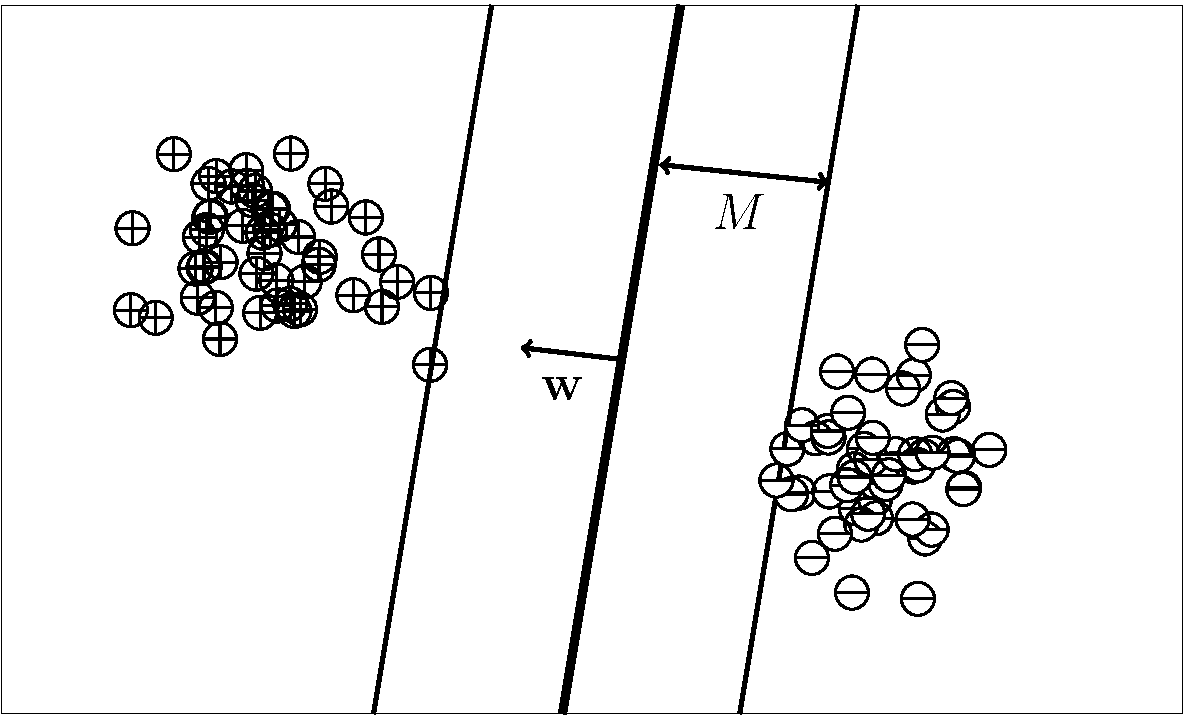
\includegraphics[width=0.5\textwidth]{aprendizaje/svm4margen} & 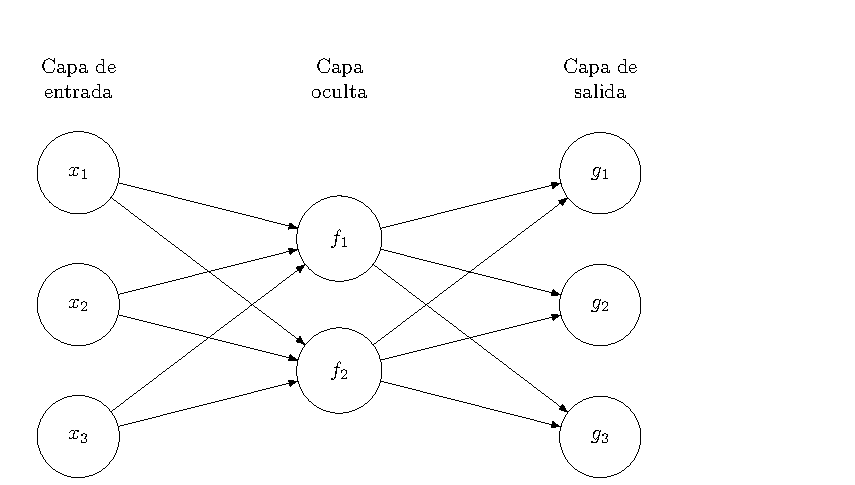
\includegraphics[width=0.6\textwidth]{aprendizaje/red_ff_funcionamiento_0} \\
    [-1.5ex] Máquinas de Vectores de Soporte (SVM)  & Redes Neuronales Feedforward (FF) \\
    %\multicolumn{3}{C{0.5\linewidth}}{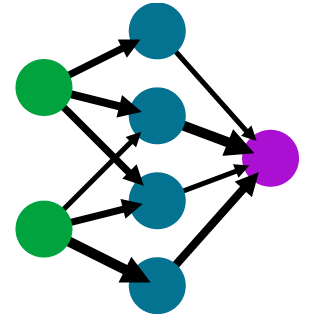
\includegraphics[scale=0.2]{intro/work/cnc}}
    %[-1.5ex] \multicolumn{3}{C{0.5\linewidth}}{Clasificador Neuronal Competitivo (CNC)}
  \end{tabular}
  \\
  
  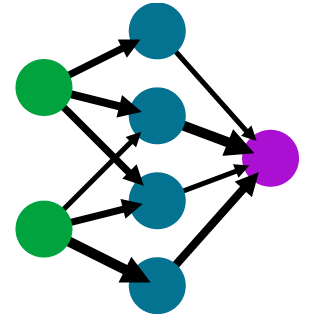
\includegraphics[scale=0.18]{intro/work/cnc}\\
  Clasificador Neuronal Competitivo (CNC)
\end{myframe}


\subsection{Modelos para comparar}
\begin{frame}
\frametitle{Modelo: Máquinas de Vectores de Soporte (SVM) }
\centering
   \begin{tabular}{C{0.5\linewidth}C{0.5\linewidth}}
      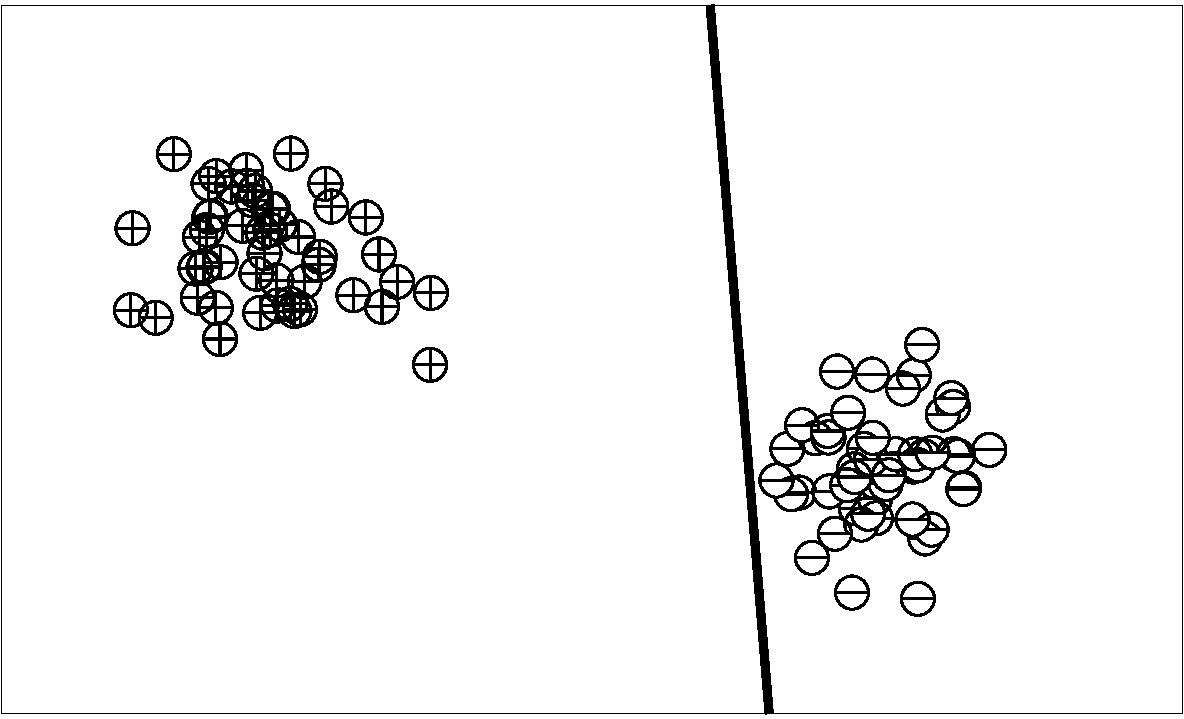
\includegraphics[width=0.5\textwidth]{aprendizaje/svm1} &  
      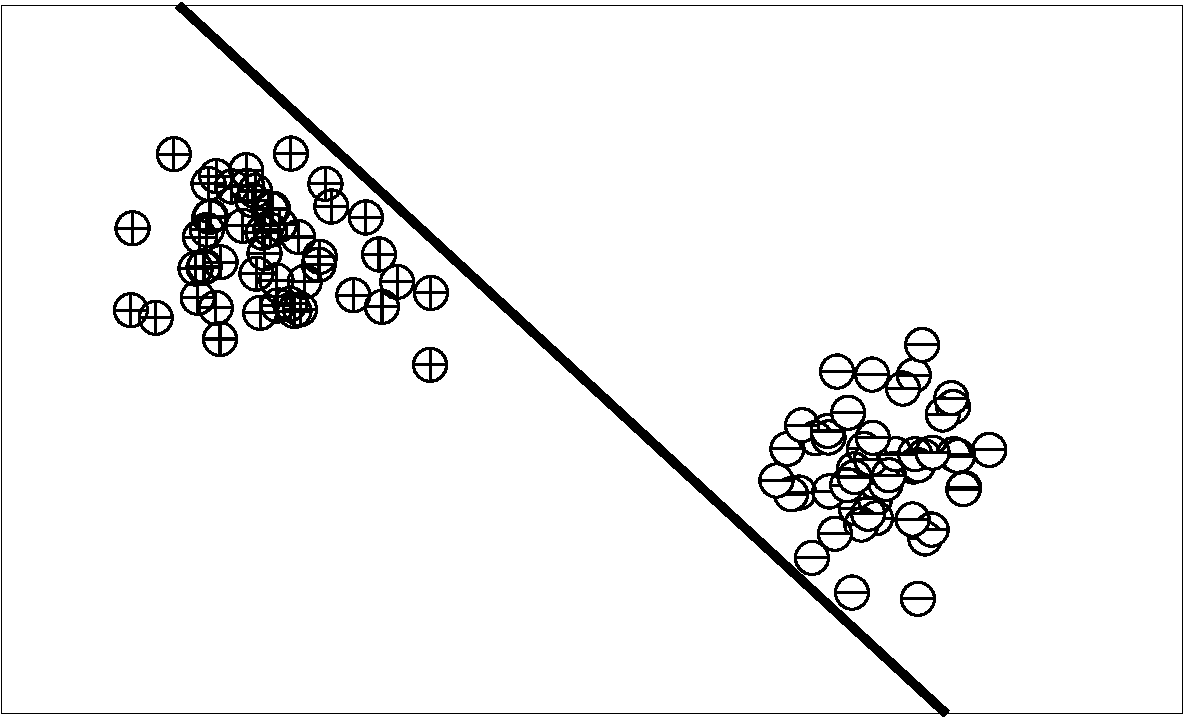
\includegraphics[width=0.5\textwidth]{aprendizaje/svm2}  \\
      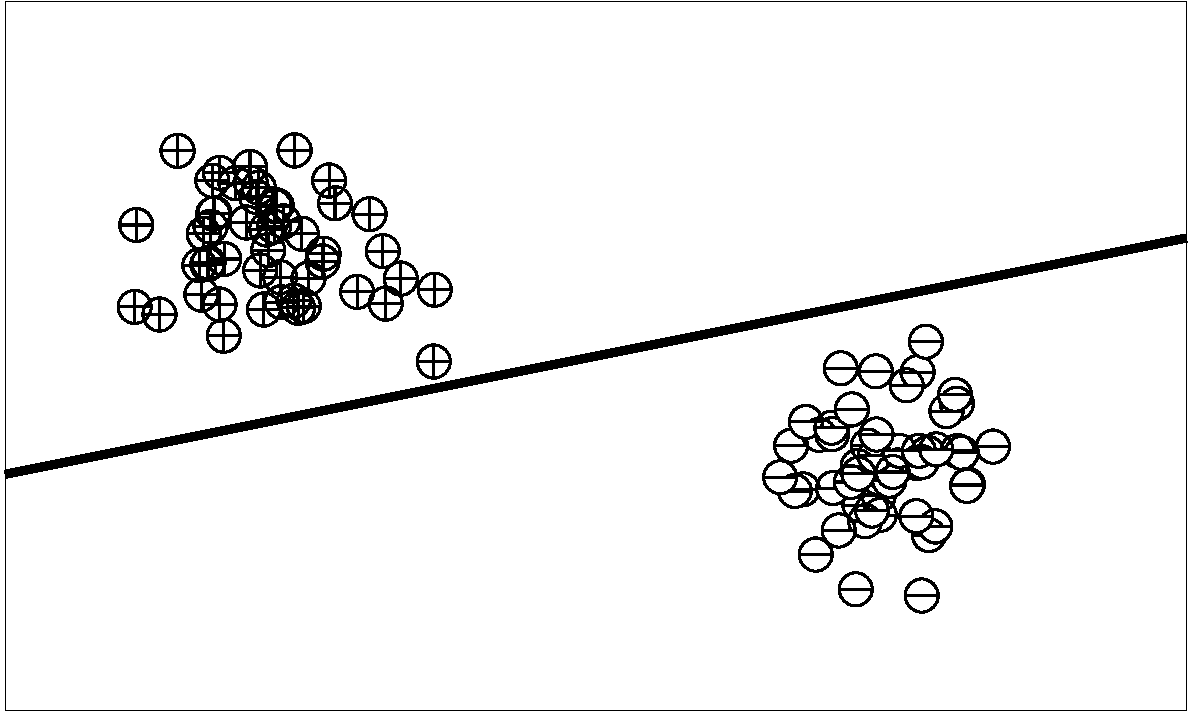
\includegraphics[width=0.5\textwidth]{aprendizaje/svm3} &    
      \includegraphics<1>[width=0.5\textwidth]{aprendizaje/svm4}
      \includegraphics<2>[width=0.5\textwidth]{aprendizaje/svm4margen}
\end{tabular}
\vspace{-5pt}
\uncover<2>{
\begin{block}{}
\vspace{-9pt}
\centering
% \begin{equation*}
% \vspace{-4pt}
%\text{Entrenamiento:} \quad \Max_{\ve{w}} M
%\end{equation*}
Entrenamiento = Separar clases y maximizar el margen M
\end{block}
}
\end{frame}


\subsection{Redes Neuronales Feedforward (FF)}
\begin{myframe}
\frametitle{Redes neuronales feedforward (FF)}
\centering
\includegraphics<1>[width=\linewidth]{aprendizaje/red_ff_funcionamiento_0}
\includegraphics<2>[width=\linewidth]{aprendizaje/red_ff_funcionamiento_1}
\includegraphics<3>[width=\linewidth]{aprendizaje/red_ff_funcionamiento_2}
\includegraphics<4>[width=\linewidth]{aprendizaje/red_ff_funcionamiento_3}
\includegraphics<5>[width=\linewidth]{aprendizaje/red_ff_funcionamiento_0}
\blockitemize{Grafo de computación}{
\item Ocultas y salida: Dinámica de la red
\item Entrenamiento con algoritmo Backpropagation
}
\end{myframe}


\subsection{Experimentos}
\begin{frame}
\frametitle{Setup experimentos}
\begin{columns}
  \begin{column}{0.7\textwidth}
    \esquemavalidacion{0.5}
  \end{column}
  \begin{column}{0.23\textwidth}
  \vspace{-60pt}
  \begin{block}{Modelos}
    \begin{itemize}
    \item SVM
    \item CNC
    \item CNC*
    \item FF
    \end{itemize}
  \end{block}
  \end{column}
\end{columns}
  \vspace{-17pt}
\begin{block}{}
\centering
\begin{itemize}
\item Pruebas preliminares para determinar parámetros: 30 corridas por cada configuración
\item Pruebas finales con mejores parámetros: 500 corridas, mejor configuración
\end{itemize}
\end{block}

\end{frame}

\subsection{Resultados}
\begin{myframe}
\frametitle{Resultados preliminares: CNC, base de datos LNHG}
\begin{columns}
\begin{column}{0.7\textwidth}
\centering
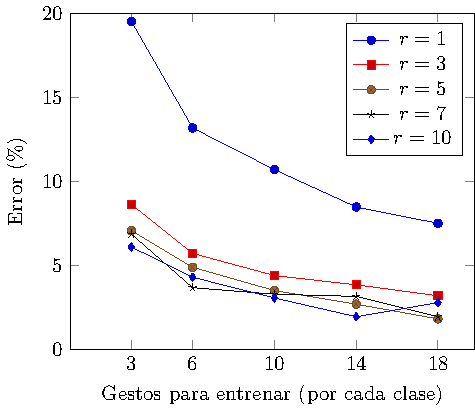
\includegraphics[scale=1]{results/defense_cnc_n}
\
\end{column}
\begin{column}{0.3\textwidth}
%\begin{block}{Detalles}
  \begin{itemize}
  \centering
%  \item p = Gestos usados para entrenar por clase
  \item Total de gestos: 720 
  \item 20 gestos por clase (36 clases)
  \item Error = Porcentaje de gestos clasificados incorrectamente
  \item r = Cantidad de redes del CNC
  %\item 30 corridas con cada configuración
  \end{itemize}
%\end{block}
\end{column}
\end{columns}

\end{myframe}

\begin{myframe}
\frametitle{Resultados preliminares: CNC*, base de datos LNHG}
\begin{columns}
\begin{column}{0.7\textwidth}
\centering
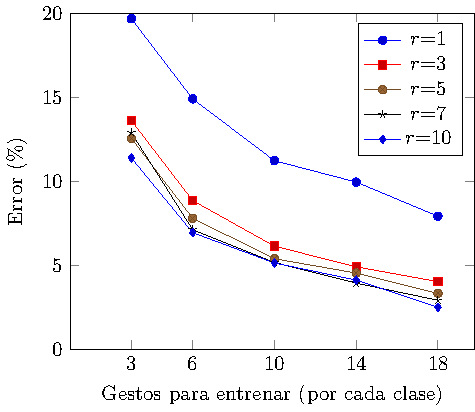
\includegraphics[scale=1]{results/defense_cnc_u}
\end{column}
\begin{column}{0.3\textwidth}
%\begin{block}{Detalles}
  \begin{itemize}
  \centering
%  \item p = Gestos usados para entrenar por clase
  \item Total de gestos: 720 
  \item 20 gestos por clase (36 clases)
  \item Error = Porcentaje de gestos clasificados incorrectamente
  \item r = Cantidad de redes del CNC
  %\item 30 corridas con cada configuración
  \end{itemize}
%\end{block}
\end{column}
\end{columns}

\end{myframe}

\begin{myframe}
\frametitle{Resultados preliminares: SVM, base de datos LNHG}
\begin{columns}
\begin{column}{0.7\textwidth}
\centering
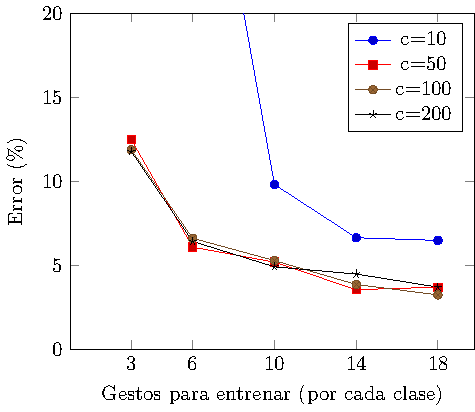
\includegraphics[scale=1]{results/defense_svm}
\end{column}
\begin{column}{0.3\textwidth}
%\begin{block}{Detalles}
  \begin{itemize}
  \centering
%  \item p = Gestos para entrenar por clase
  \item Total de gestos: 720 
  \item 20 gestos por clase (36 clases)
  \item Error = Porcentaje de gestos clasificados incorrectamente
  \item c = Costo clasificación incorrecta
  
  %\item 30 corridas con cada configuración
  \end{itemize}
%\end{block}
\end{column}
\end{columns}

\end{myframe}


\begin{frame}
\frametitle{Resultados finales: Base de datos LNHG, 500 corridas}
\vspace{-13pt}
\begin{table}[h]
\centering
%\small
\begin{tabulary}{\linewidth}{|C{0.22\linewidth}|C{0.22\linewidth}|C{0.22\linewidth}|C{0.22\linewidth}|}
\hline Clasificador & Parámetros &  Error $= \mu$ ($\sigma$) \\ 
%\hline SVM (Lineal) & $c=200$, $n=128$ & SMO &  11.76 \% (0.080) \\ 
%\hline SVM (Gaussiano) & $c=100$, $\sigma=64$, $n=128$ & SMO & 11.44 \%  (0.063)  \\ 
\hline SVM & $c=100$, $n=128$ & 11.76 \%  (0.080)  \\ 
\hline CNC & $h=50$, $r=10$ $n=32$ & 5.92 \%  (0.088)\\ 
\hline CNC* & $h=50$, $r=10$ & 11.29 \% (0.092) \\ 
\hline FF & $h=100,n=16$ & 18.60 \% (0.158) \\ 
%\hline Template & $n=16$ & - & $\mu= 53.77$\% (0.050) \\ 
\hline 
\end{tabulary}
\end{table}

\vspace{-10pt}
\blockitemize{Ventajas del CNC}{
\item Menos sensible a la cantidad de ejemplares de entrenamiento
\item Puede utilizarse sin re-muestreo (CNC*)
}


\end{frame}


%\begin{myframe}
%\frametitle{Resultados finales: Base de datos Celebi2013}
%
%\begin{table}[h]
%\centering
%%\small
%
%\begin{tabulary}{\linewidth}{|C{0.22\linewidth}|C{0.22\linewidth}|C{0.22\linewidth}|C{0.22\linewidth}|}
%\hline Clasificador & Parámetros & Entrenamiento & \cc \, $= \mu$ ($\sigma$) \\ 
%\hline SVM (Lineal) & $c=100,n=16$ & SMO &  100 \% (0.002) \\ 
%\hline SVM (Gaussiano) & $n=16,\sigma=64,c=100$ & SMO & 100\% (0.005)  \\ 
%\hline CNC & $h=70,r=10,n=16$ & CNC, $\alpha=0.5$ & 100\% (0.015) \\ 
%\hline CNC* & $h=70$, $p=5$ & CNC, $\alpha=0.5$ & 100\% (0.022)  \\ 
%\hline FF & $h=100,n=16$ & iRprop+ &  100 \%  (0.028) \\ 
%\hline Template & $n=16$ & - & 100\% (0.006) \\ 
%\hline Celebi2013 &  & DTW adaptativo & 97\% \\ 
%\hline 
%\end{tabulary}
%\end{table}
%
%\end{myframe}


\subsection{Conclusiones}
%\begin{myframe}
%\frametitle{Desempeño del CNC y comparación con otros métodos}
%
%\end{myframe}

\begin{myframe}
\frametitle{Puntos a mejorar}
\begin{itemize}
\item El CNC pierde toda información de la secuencia de direcciones \\ 
$\rightarrow$ “Colisiones”: gestos distintos con la misma distribución de direcciones
\item Pruebas de tiempo real no satisfactorias \\
$\rightarrow$ Requiere segmentación de buena calidad
\item Pocos gestos \\
$\rightarrow$ Las únicas bases de datos de gestos con la mano son de imágenes/video
\end{itemize}
\end{myframe}

\begin{myframe}
\frametitle{Trabajo futuro}
\begin{itemize}
\item Reconocimiento en tiempo real
\item “Spotting”: reconocer principio y fin del gesto
\item Grabar más ejemplos y clases de gestos
\item Utilizar métodos de bagging con todos los algoritmos
\item Probar otras características (Coeficientes de DFT normalizados o momentos de Hu).
\end{itemize}
\end{myframe}

\subsection{}
\begin{myframe}
\frametitle{Fin}
\begin{center}
{\Huge Gracias!}
\end{center}
\end{myframe}
